\section{Zielsetzung}
Ziel des Experimentes ist, anhand einer elektrischen Schaltung das Verhalten eines schwingfähigen Systems zu erkunden. 
Betrachtet werden eine reine Schwingung und eine erzwungene Schwingung jeweils mit Dämpfung.

\section{Theorie}
\label{sec:Theorie}
% Kann ein schwingfähiges System, nachdem es angeregt wurde, ohne weiteren Einfluss von außen oszillieren, so handelt es sich um eine freie Schwingung.
% Bleibt der von außen gegebene Antrieb über lange Zeit erhalten, so handelt es sich um eine erzwungene Schwingung. \cite{kuchen}
\subsection{Freie Schwingung mit Dämpfung}
\label{sec:theorie1}
\begin{figure}[h]
	\centering
	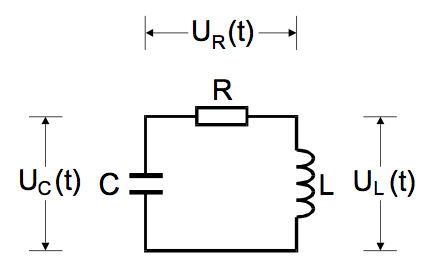
\includegraphics[width=0.4\textwidth]{Bilder/Maschenfoto1.png}
	\caption{Schaltskizze des untersuchten Systems. \cite{v354}}
	\label{fig:schaltkreis_rein}
\end{figure}
Das System wird in \ref{fig:schaltkreis_rein} gezeigt, die jeweiligen Spannungsabfälle und -quellen sind eingezeichnet.
Nach der Zweiten Kirchhoffschen Regel ist in einer Masche die Summe aller Spannungen gleich Null. 
Daraus folgt für das System
\begin{equation}
	U_\text{R}(t)+U_\text{C}(t)-U_\text{L}(t)=0
\end{equation}
unter Beachtung der Stromrichtung der Komponenten.
Mit den allgemeinen Formeln für die Spannung der jeweiligen Schaltkreiskomponente,
\begin{align}
	U_\text{R}(t) &= \text{R} I(t)\\
	U_\text{C}(t) &= \frac{Q(t)}{\text{C}} \\
	U_\text{L}(t) &= -\text{L}\frac{\mathup{d}I(t)}{\mathup{d}t},
\end{align}
und der Substitution
$I=\frac{\mathup{d}Q(t)}{\mathup{d}t}$,
wird das System mit der Differentialgleichung für den Strom $I(t)$ beschrieben.
Es gilt
\begin{equation}
	\frac{\mathup{d^2}I(t)}{\mathup{d}t^2}+\frac{\mathup{R}}{\mathup{L}}\frac{\mathup{d}I(t)}{\mathup{d}t}+\frac{1}{\mathup{LC}}.
\end{equation}
Die allgemeine Lösung der Differentialgleichung ist
\begin{equation}
	I(t) = A_1\cdot e^{\mathup{\omega_1}t} +A_2\cdot e^{\mathup{\omega_2}t}
	\label{eq:allgloesung}
\end{equation}
mit der Abkürzung
\begin{equation}
	\mathup{\omega_{1,2}}= -\frac{\mathup{R}}{2\mathup{L}}\pm\sqrt{\underbrace{\frac{\mathup{R^2}}{4\mathup{L^2}}-\frac{1}{\mathup{LC}}}_{\text{Diskriminante}}}.
	\label{eq:allomega}
\end{equation}
Durch den Radikanten als Diskriminante sind drei Fälle möglich.

%\subsubsection{Schwingfall}
Für $\frac{\mathup{R^2}}{4\mathup{L^2}}-\frac{1}{\mathup{LC}}<0$ \\
ist $\omega$ in \eqref{eq:allomega} komplex.
Es ergibt sich als Lösung für $\omega$
\begin{equation}
	\mathup{\omega_{1,2}}= -\frac{\mathup{R}}{2\mathup{L}}\pm i\sqrt{\frac{1}{\mathup{LC}}-\frac{\mathup{R^2}}{4\mathup{L^2}}}
\end{equation}
mit
\begin{equation}
	I(t) = e^{-\frac{\mathup{R}}{2\mathup{L}}\,t}(A_1 \sin\Bigl(\sqrt{\frac{1}{\mathup{LC}}-\frac{\mathup{R^2}}{4\mathup{L^2}}}\, t\Bigr)+A_2 \cos\Bigl(\sqrt{\frac{1}{\mathup{LC}}-\frac{\mathup{R^2}}{4\mathup{L^2}}}\,t\Bigr)\
	\label{eq:schwingloesung}
\end{equation}
%\subsubsection{aperiodischer Grenzfall}
Für $\frac{1}{\mathup{LC}}=\frac{\mathup{R^2}}{4\mathup{L^2}}$ \\
verschwindet der Wurzelterm von $\omega$ in \eqref{eq:allomega}.
Die so vereinfachte Lösung heißt aperiodischer Grenzfall und beschreibt den ausgezeichneten Stromverlauf, der nach Auslenkung die Ruhelage - hier $I(t)=0 \quad\forall t$ - am Schnellsten wieder erreicht.\\
Zur allgemeinen Lösung für diesen Fall wird eine zusätzliche Fundamentallösung benötigt.
Es gilt
\begin{equation}
	I(t) = A_1 e^{-\frac{\mathup{R}}{2\mathup{L}}\,t}+A_2 t e^{-\frac{\mathup{R}}{2\mathup{L}}\,t}
\end{equation}
%\subsubsection{Kriechfall}
Für $\frac{\mathup{R^2}}{4\mathup{L^2}}-\frac{1}{\mathup{LC}}>0$ \\
ist der Wurzelterm von $\omega$ in \eqref{eq:allomega} rein reell.
Die so vereinfachte Lösung ist eine exponentielle Abnahme.
Es gilt
\begin{equation}
	I(t)= A_1 e^{\omega_1 t} + A_2 e^{\omega_2 t}
\end{equation}
\begin{figure}
	\centering
	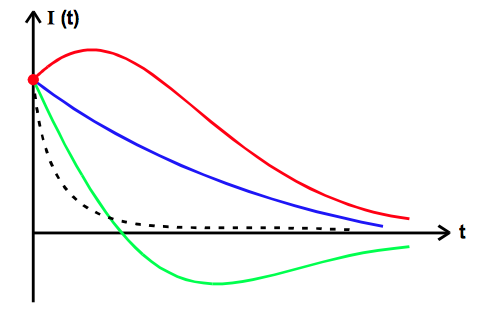
\includegraphics[width=0.5\textwidth]{Bilder/Loesungsform.png}
	\caption{Darstellung aller möglichen Stromverläufe. \cite{v354}}
\end{figure}

\subsection{Erzwungene Schwingung mit Dämpfung}
\label{sec:theorie2}
\begin{figure}[ht]
	\centering
	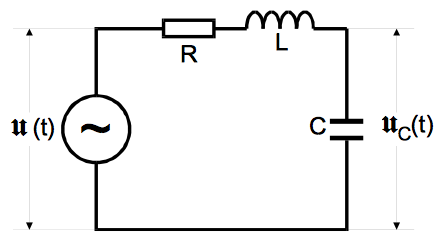
\includegraphics[width=0.4\textwidth]{Bilder/Maschenfoto2.png}
	\caption{Schaltskizze des untersuchten Systems. \cite{v354}}
	\label{fig:schaltkreis_erzwungen}
\end{figure}
In diesem System wird die Spannung $U_\text{C}$, die am Kondensator anliegt, betrachtet.
Analog zu Abschnitt \ref{sec:theorie1} beschreibt die Gleichung
\begin{equation}
	U_\text{R}(t)+U_\text{C}(t)-U_\text{L}(t)=U(t)
\end{equation}
mit der Generatorspannung $U(t)=U_0 e^{i\omega t}$ das System.
Mit der Substitution
$I=\frac{\mathup{d}Q(t)}{\mathup{d}t}$ und $U_\text{C}(t) = \frac{Q(t)}{\text{C}}$,
wird das System mit der Differentialgleichung 
\begin{equation}
	\mathup{LC}\frac{\mathup{d^2}U_\mathup{C}}{\mathup{d}t^2} +\mathup{RC}\frac{\mathup{d}U_\mathup{C}}{\mathup{d}t} +U_\mathup{C} =U_0 e^{i\omega t}
	\label{eq:DGLerzw}
\end{equation}
beschrieben.
Die Lösung dieser inhomogenen Differntialgleichung setzt sich aus homogener und inhomogener Lösung zusammen.
Es ist aus Abschnitt \ref{sec:theorie1} bekannt, dass die homogene Lösung für große Zeiten gegen Null geht.
Mithilfe des Ansatzes $U_\mathup{C}(\omega,t)= \tilde{U}_\mathup{\omega}(\omega)\cdot e^{i\omega t}$,
$\tilde{U}_\mathup{\omega}(\omega)\in\mathbb{C}$ ist die komplexe Amplitude mit Phasenwinkel $\mathup{arg}(\tilde{U}_\mathup{\omega})=\phi$ und Betrag $|\tilde{U}_\mathup{\omega}|=U_\mathup{\omega}$, ist die inhomogene Lösung von Differentialgleichung \eqref{eq:DGLerzw}
\begin{align}
	U_0 &= - \mathup{LC}\omega^2 \tilde{U}_\mathup{\omega}(\omega) + i\omega\mathup{RC}\tilde{U}_\mathup{\omega}(\omega) + \tilde{U}_\mathup{\omega}(\omega)\\
	\intertext{mit}
	U_\mathup{\omega}&= U_0\frac{\sqrt{(1 − \mathup{LC}\omega^2)^2 +\mathup{ω^2R^2C^2}}}{\Bigl(\sqrt{(1 − \mathup{LC}\omega^2)^2 +\mathup{ω^2R^2C^2}}\Bigr)^2}\label{eq:yes}\\
	\mathup{tan}(\phi) &= \frac{\mathup{Im}(\tilde{U}_\mathup{\omega})}{\mathup{Re}(\tilde{U}_\mathup{\omega})}=\frac{−ω\mathup{RC}}{1 − \mathup{LC}ω2}
\end{align}
Aus \eqref{eq:yes} und dem gewählten Ansatz folgt für die Amplitude der Lösungsfunktion der Differentialgleichung \eqref{eq:DGLerzw}
\begin{equation}
	|U_\mathup{C}| = \frac{U_0}{\sqrt{(1 − \mathup{LC}\omega^2)^2 +\mathup{ω^2R^2C^2}}} 
\end{equation}

% Es fehlt eine vernünftige Liste der obenstehenden Formeln, Resonanzfall, Grenzfälle, Neue Frequenz,
% Schwingformel nach Thomson, Abnahmezeit, Spannungsüberhöhung

% Geld ist ja bekanntlich im Portmonee. Da steckt man es rein und es kommt nicht da raus. Außer man kauft etwas davon, zum Beispiel Suppe. (In der Tüte oder nicht, dass ist in diesem Fall egal). Aber wie teuer ist Suppe?

% Jeder kennt das berühmte Bild von einer Suppe. Es war aber nicht in einer Tüte, nein, nein, es war in einer (bunten bzw. roten) Dose! Und hätte man die Dose geöffnet? Hätte es jemand gemacht, man könnte es schreiben. Hat aber Keiner. Deswegen kann man es schwer sagen. Und Suppe: Man kann sie auch mit dem Geld bezahlen.

% Das durchschnittliche Einkommen eines deutschen Haushaltes beträgt etwa 2700 €, nach Abzug aller relevanten und laufenden Kosten (Steuern, Miete et cetera) noch etwa 1350 €.

% Man kann aber nicht alles das Geld für die Suppe (oder z.B. Trockenobst) ausgeben. Kann man natürlich, aber da gibt es ja noch andere Sachen.

% Geld wächst ja bekanntlich auch nicht am Baum (genau wie Suppe), schon wieder etwas das auffällt. Aber Suppe kann man zumindest herstellen. Eine durchschnittliche Suppenküche stellt viel Suppe her, zum Beispiel um sie zu verkaufen oder zu vermieten. Aber wie wird die Suppe überhaupt zu Trockensuppe gemacht?

% Die Suppe besteht bestimmt so aus 20\% Wasser, vielleicht mehr. In der Tüte, da kommt noch Wasser zur Suppe rein, dann ist es Suppe. Also Wasser zum Suppenmehl. Typisch deutsch? Weit gefehlt, auch in China gibt es mittlerweile mehrere Prozent Suppe aus dem Kochbeutel. Auch in Norwegen oder Albanien.

% Aber wieso eigentlich ausgerechnet Suppe? Warum nicht zum Beispiel Gänsebraten oder so was? Ganz einfach: Suppe enthält viele Vitamine. So wie Saft. Und die erstaunliche Parallele: Saft und Suppe kann man beides kalt essen. Es geht bei Suppe also vielmehr um die Temperatur (in °C oder Kelvin, aber nicht in Fahrenheit (oder so)). Probieren Sie es selber aus: Suppe ist ein Gericht, dass am besten kalt serviert wird.

% Genauso wie Geld. Denn das gibt es (es ist also) meistens im Portmonee.
